% Autor: Lukas Deeken
% Letzte Bearbeitung: 01.05.2022

\chapter{Elektrische Systeme}
Hier Geht mein dank an die Alumni aus dem Bereich der Elektrotechnik die diese ganze Reise mit ihrer fachlichen Referenz und beispiellosen Motivation erst möglich gemacht habe. Hervorzuheben ist auch das schier endlose mas an gedult in Anbetracht der Steilen Lernkurve innerhalb des Teams. Besonders hervorzuheben sind hierbei Leon Löser, Eric Gorkow und Axel Lange. Danke euch.
\acfirst{IMD}
\section{Akkumulator}
Akkumulaotr layout und connections
	AMS DCDC IMD TS Sensors AIR etc. mit visio

\subsection{AMS Master und Slave}
Layout welche Funktionen sind wo, wozu gibt es Funktionen etc.
Sprich Precharge auf AMS Master

\subsubsection{Precharge}
Der Precharge verhindert einen Funkenschlag und damit das verschweißen der Akku Isolationsrelais beim Schließen. Dies wird erreicht indem der Zwischenkreis bereits vor dem Durchschalten der AIR`s auf die Akkuspannung aufgeladen wird. Anhand des folgenden Blockschaltbildes lassen sich die einzelnen funktionellen Blöcke herausarbeiten.

\begin{figure}
	\centering
	\includegraphics[width=0.7\linewidth]{"bilder/Precharge Blockschaltbild"}
	\caption{}
	\label{fig:precharge-blockschaltbild}
\end{figure}

Kernelement ist die Verbindung der positiven Seite des Zwischenkreises mit der positiven Seite des Akkumulators über ein mechanisches Relais, und die Überwachung selbigens. Diese kann nicht mit einer AUX Beschaltung umgesetzt werden, da Relais in diesem Leistungsbereich idR nicht mit derartigen Funktionen ausgerüstet sind. Eine Besonderheit bei dem gewählten Relais ist die geringe Baugröße, aber auch ein damit einhergehendes niedriges Stromrating, so das der Einschaltstrom des Relais der Strom sehr klein gehalten werden muss. Aus diesem Grunde bedarf es einer Stromquelle welche zu beginn einen niedrigen Strom liefert, und diesem dann nach dem erfolgten schalten anhebt. Nun zur Klärung der einzelnen funktionellen Gruppen und der Schaltzustände.

\begin{figure}
	\centering
	\includegraphics[width=0.7\linewidth]{"bilder/Precharge Blockschaltbild Detail"}
	\caption{}
	\label{fig:precharge-blockschaltbild-detail}
\end{figure}

Der Precharge schaltet durch sobald SC\textsubscript{end} high wird. Dies führt zum Durchschalten des Relais. Nun fließt ein Strom über M1 zum Relais, bei der Verschaltung von M1 und R54 handelt es sich um eine Konstantstromquelle welche 0,05A liefert. Wie diese Art von Schaltung im Detail funktioniert ist unter \ref{sec: TSAL Logik Discharge} näher erläutert. Parallel fließt ein Strom über U3 zu C58 und lädt diesen. Nach kurzer Zeit führt dies dazu das Q10 durchschaltet, nun wird der Strom durch den Widerstand der PTC Elemente begrenzt so das der Strom auf ca. 0.6 A ansteigen kann. Die Überwachung erfolgt indem mithilfe eines DC Wandlers die Akkuspannung um 24V angehoben wird und diese über einen Optokoppler auf das Precharge Relais gelegt wird. Sobald das Relais geschlossen ist fließt somit ein Strom über U22 sodass bei PCHRG\textsubscript{ACT} eine Spannung anliegt.

Im Ausschaltmoment wird das Relais durch die Kapazität C12 für kurze Zeit offen gehalten sodass zuerst der Mosfet Q10 abschaltet und so die Schaltleistung im Relais minimiert wird.

\begin{figure}
	\centering
	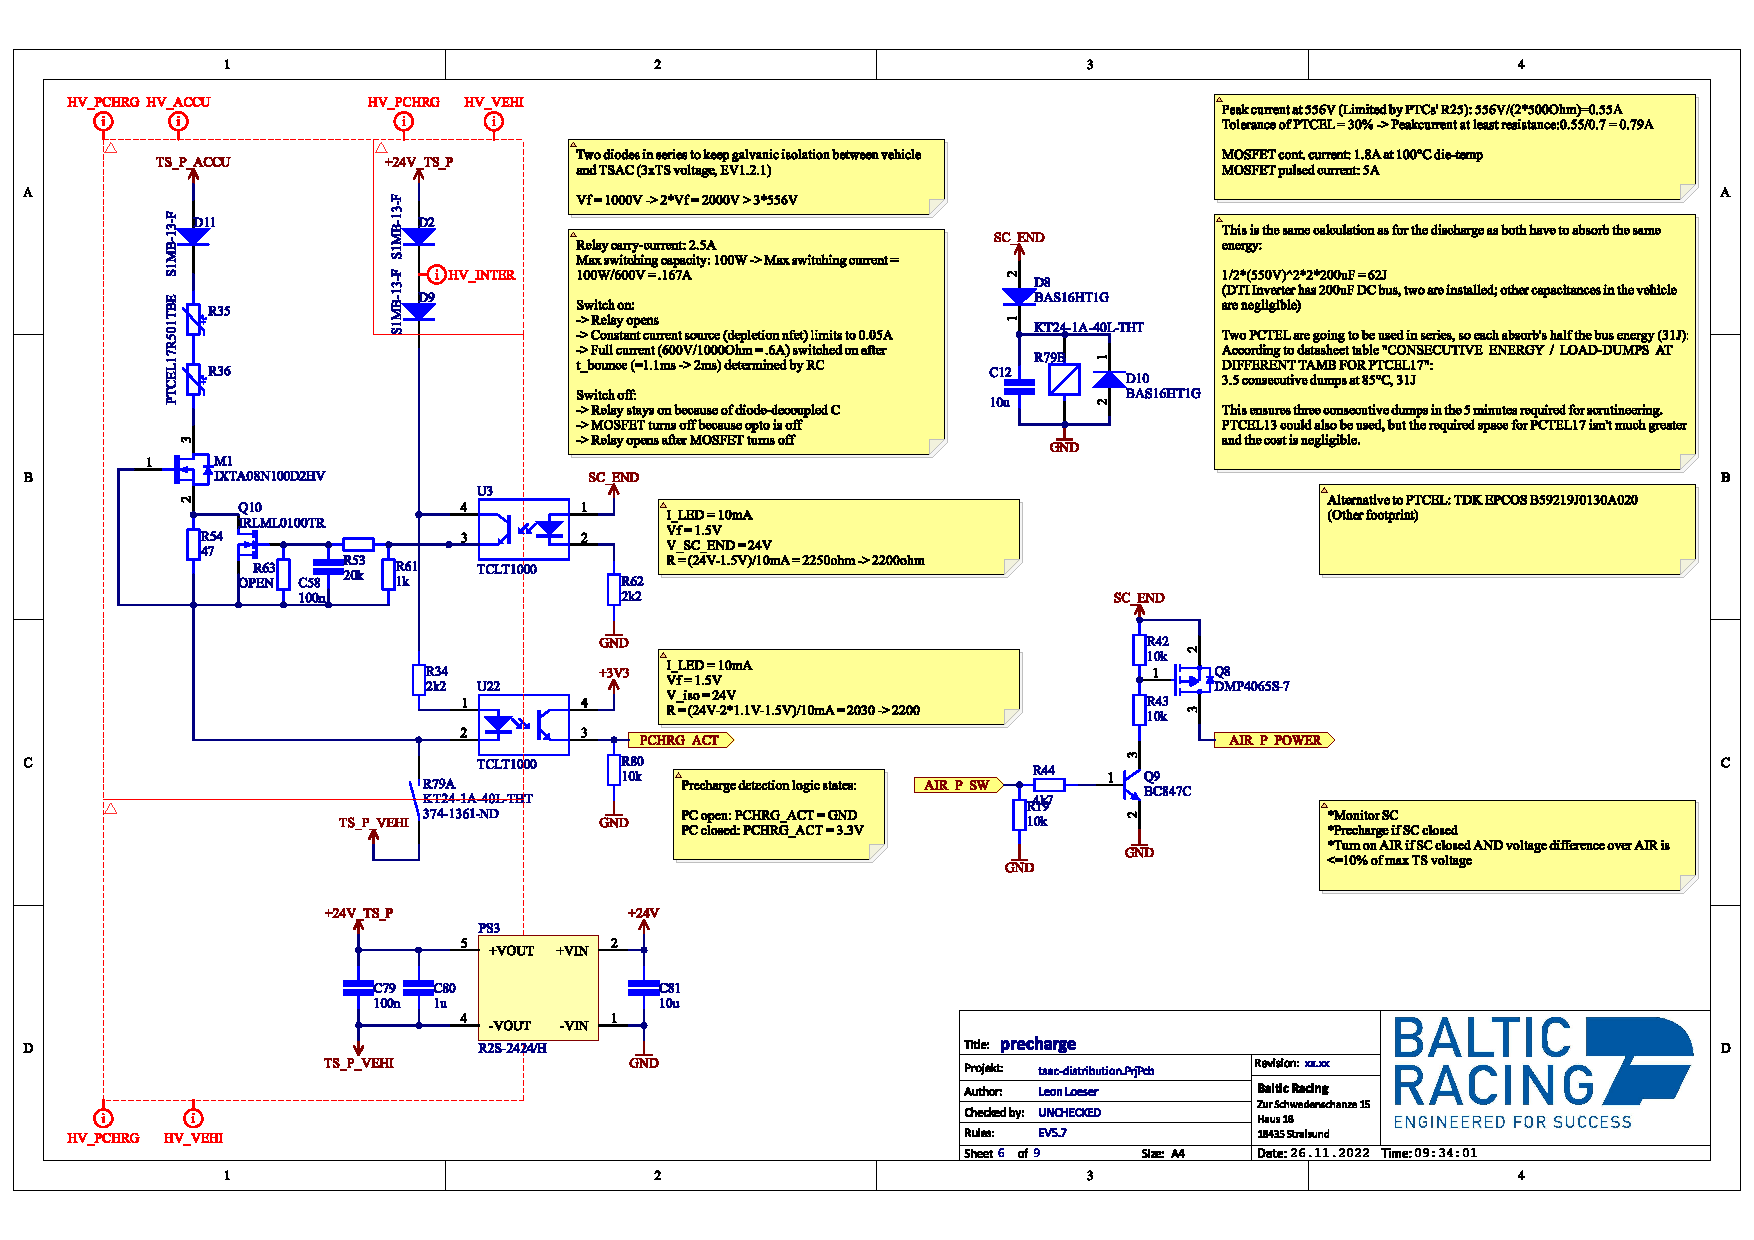
\includegraphics[width=0.7\linewidth]{bilder/Precharge_Complete}
	\caption{}
	\label{fig:prechargecomplete}
\end{figure}

\subsubsection{AIR Detection}

\begin{figure}
	\centering
	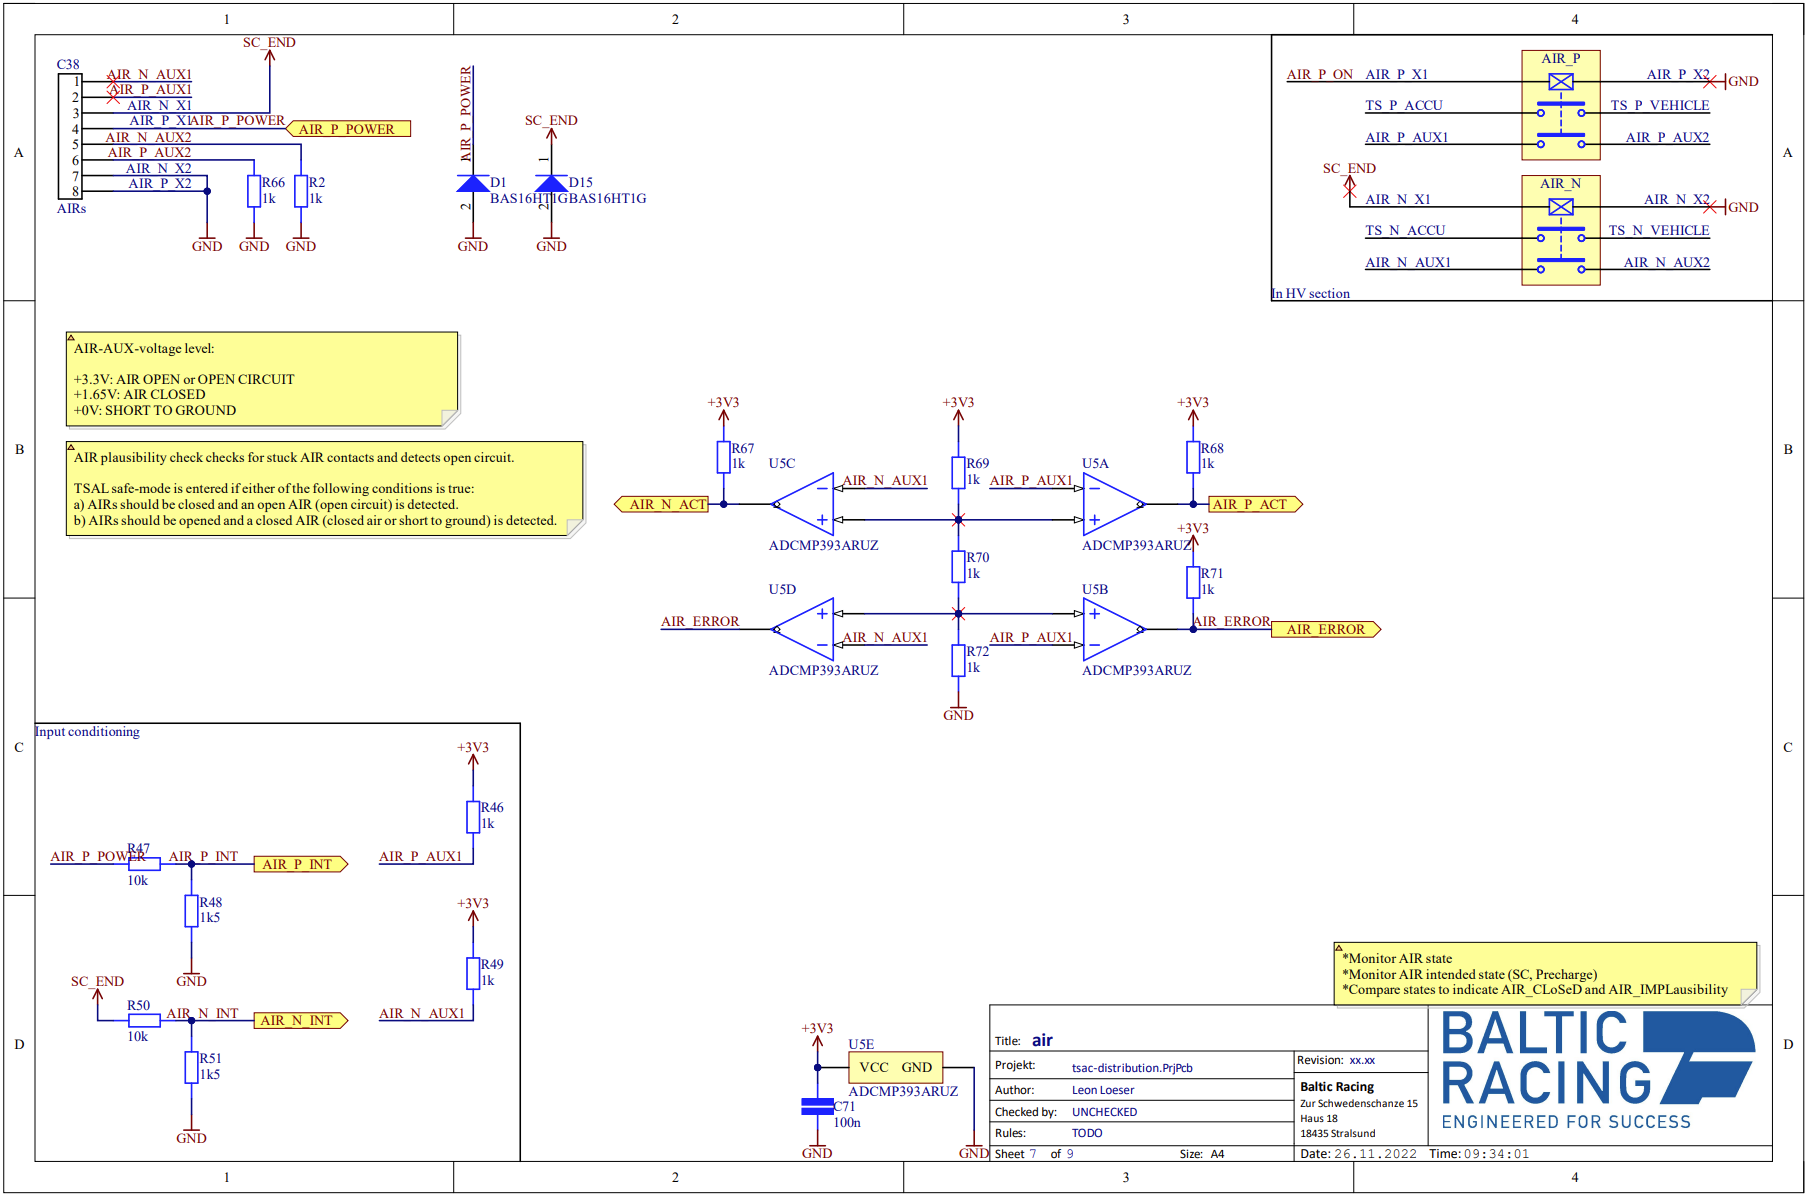
\includegraphics[width=0.7\linewidth]{bilder/AIR_conditioning}
	\caption{}
	\label{fig:airconditioning}
\end{figure}

Sinn der AIR detection ist es die Signale vom AIR in Sinnvolle Logikpegel umzusetzen welche im späteren verlauf weiter verwendet werden können. Oben rechts auf der Schematik sind die AIRs dargestellt. Relevant sind dabei die X Signale welche den Schaltzustand des Relais kontrollieren und die AUX Signale welche den Schaltzustand überwachen. Die AUX Signale werden mit 3,3V über einen Gleichwertigen 1 kOhm Spannungsteiler versorgt, so das bei geöffnetem Relais die 3,3V an AUX 1 anliegen, bei geschlossenem Relais durch den Spannungsteiler 1,65V und bei einem Kurzschluss in der Signalleitung zu Masse 0V anliegen. Diese Spannungspegel werden jetzt in einer komparatorschaltung verglichen. Die oben beiden Komparatoren geben ein High Signal aus wenn die Spannung an den AUX Kontakten kleiner ist als die Referenzspannung und damit die Relais geschlossen oder auf Masse kurzgeschlossen sind. Die beiden unteren Komparatoren geben ein Low Signal aus wenn die Spannung größer ist als die Referenzspannung und damit das Relais geschlossen oder geöffnet ist. Sofern also der tatsächliche zustand des Relais High ist un der Fehler Low kann zum Beispiel geschlussfolgert werden das jenes Relais geschlossen ist.

\subsubsection{AMS}
Das eigentliche Batteriemanagement wird von vom LTC 6804 übernommen. hierbei handelt es sich um eine integrierte Schaltung welche speziell für die Aufgabe des batteriemanagment von Linear Technology entwickelt wurde. Relevante aufgaben dieses Chips ist die differentielle Messung der Zellspannungen im Stack. Weiter übernimmt der IC die Temperatur Messung über 5 frei nutzbare GPIO`s welche auch ADC Funktionalität unterstützen. Zu guter Letzt wird der Chip als Treiber für Mosfets benutzt welche die Zelle auf den balancing widerstand schalten. Die notwendige Kommunikation erfolgt über einen proprietären 2 drahtigen linearen isolierten SPI Bus. Jeder Chip hat dabei 4 Adressbits zur Konfigurierung. Das Kommunikationsinterface zischen dem Iso SPI und dem SPI bus des Mikrocontroller erfolgt über den LTC6820 welcher für exakt diese Aufgabe entwickelt wurde. Mit den 5 Eingängen am Chip sind nun 11 verschiedene NTC`s auszuwerten, dies geschieht mit Hilfe eines Demuxers und eines Invertierers.

Zum Verständnis der Logik ist im folgenden einmal beispielhaft der Signalablauf dargestellt.
Die Bits SEL0 (0) und SEL1 (1) vom BMS Chip U1 gehen auf die Eingänge A und B am Demuxer U6. G2A (0) und G2B (0) sind immer auf Low gesetzt und G1 (1) immer auf High. Mit der Tabelle \ref{Demuxer_Logiktabelle} aus dem Datenblatt wird nun der Ausgang von Y0 bis Y3 bestimmt.

\begin{figure}
	\centering
	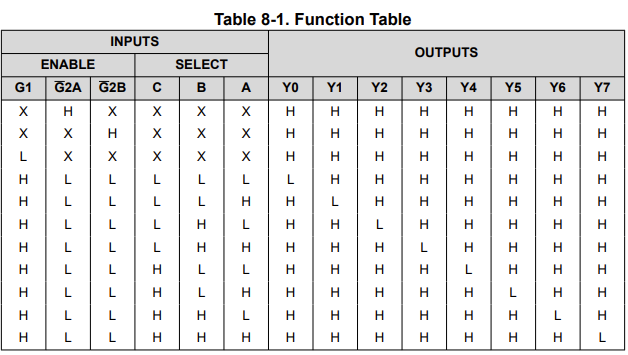
\includegraphics[width=0.3\linewidth]{bilder/AMS_demuxer_logiktabelle}
	\caption{}
	\label{Demuxer_Logiktabelle}
	\label{fig:amsdemuxerlogiktabelle}
\end{figure}

\FloatBarrier

\begin{tabular}{|c|c|}
	\hline
	Y0 & 1 \\
	\hline
	Y1 & 1 \\
	\hline
	Y2 & 0 \\
	\hline
	Y3 & 1 \\
	\hline
\end{tabular}

Diese Signale gehen nun in die beiden Invertierer U2 \& U5. Der Ausgang des Invertierer stellt die Versorgung des NTC dar.

\begin{tabular}{|c|c|}
	\hline
	NTC-sig0 & 0 \\
	\hline
	NTC-sig0 & 0 \\
	\hline
	NTC-sig1 & 1 \\
	\hline
	NTC-sig2 & 0 \\
	\hline
	NTC-sig3 & 0 \\
	\hline
	NTC-sig4 & 0 \\
	\hline
	NTC-sig5 & 0 \\
	\hline
	NTC-sig6 & 1 \\
	\hline
	NTC-sig7 & 0 \\
	\hline
	NTC-sig8 & 0 \\
	\hline
	NTC-sig9 & 0 \\
	\hline
	NTC-sig10 & 0 \\
	\hline
	NTC-sig11 & 1 \\

\end{tabular}

\begin{figure}
	\centering
	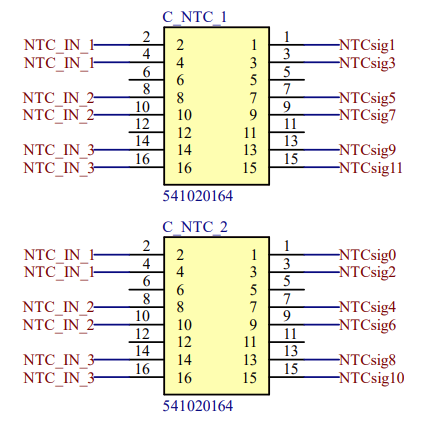
\includegraphics[width=0.3\linewidth]{bilder/AMS_NTC_steckerlayout}
	\caption{}
	\label{fig:amsntcsteckerlayout}
\end{figure}

zusammen mit dem NTC Steckerlayout ergibt dies also das an NTCin1 bis NTCin3 jeweils ein Signal von einem NTC anliegt.







\begin{figure}
	\centering
	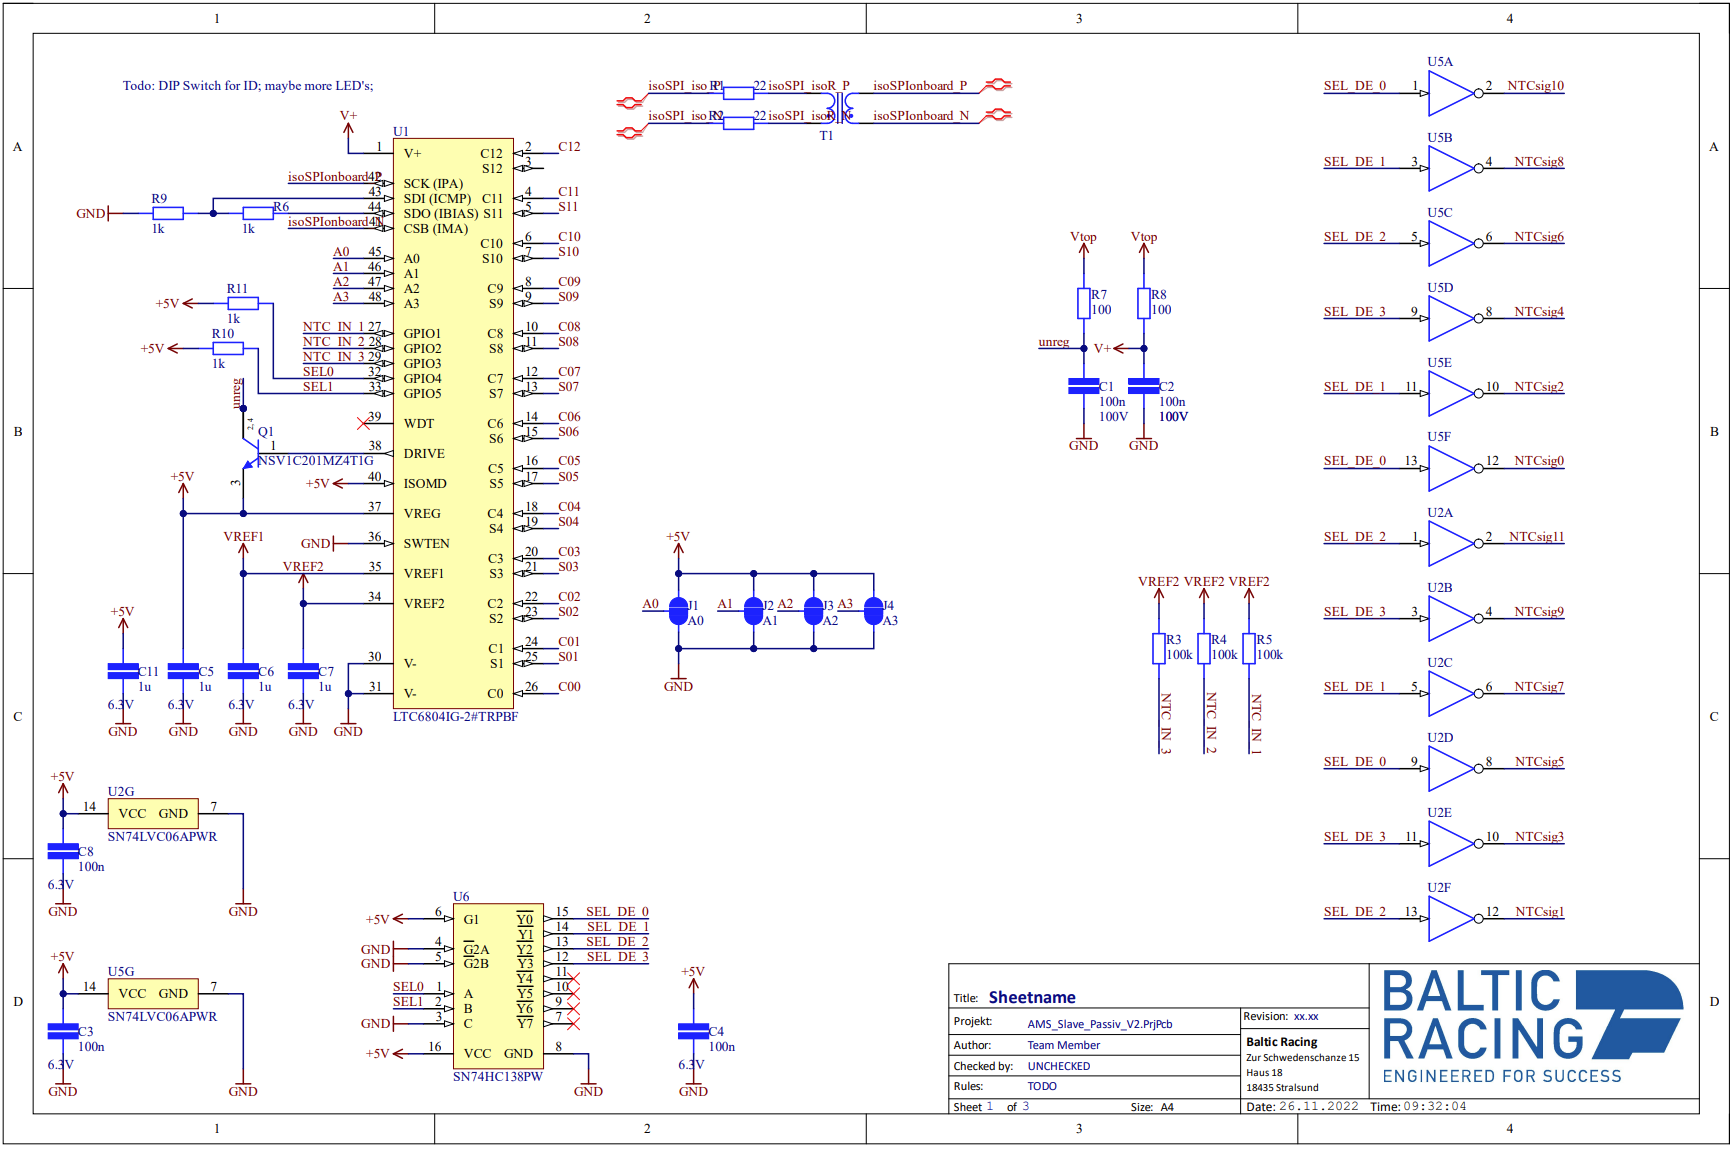
\includegraphics[width=0.7\linewidth]{bilder/AMS_slave_controller_schematic}
	\caption{}
	\label{fig:amsslavecontrollerschematic}
\end{figure}

\FloatBarrier
\subsubsection{HV Indicator}

\begin{figure}
	\centering
	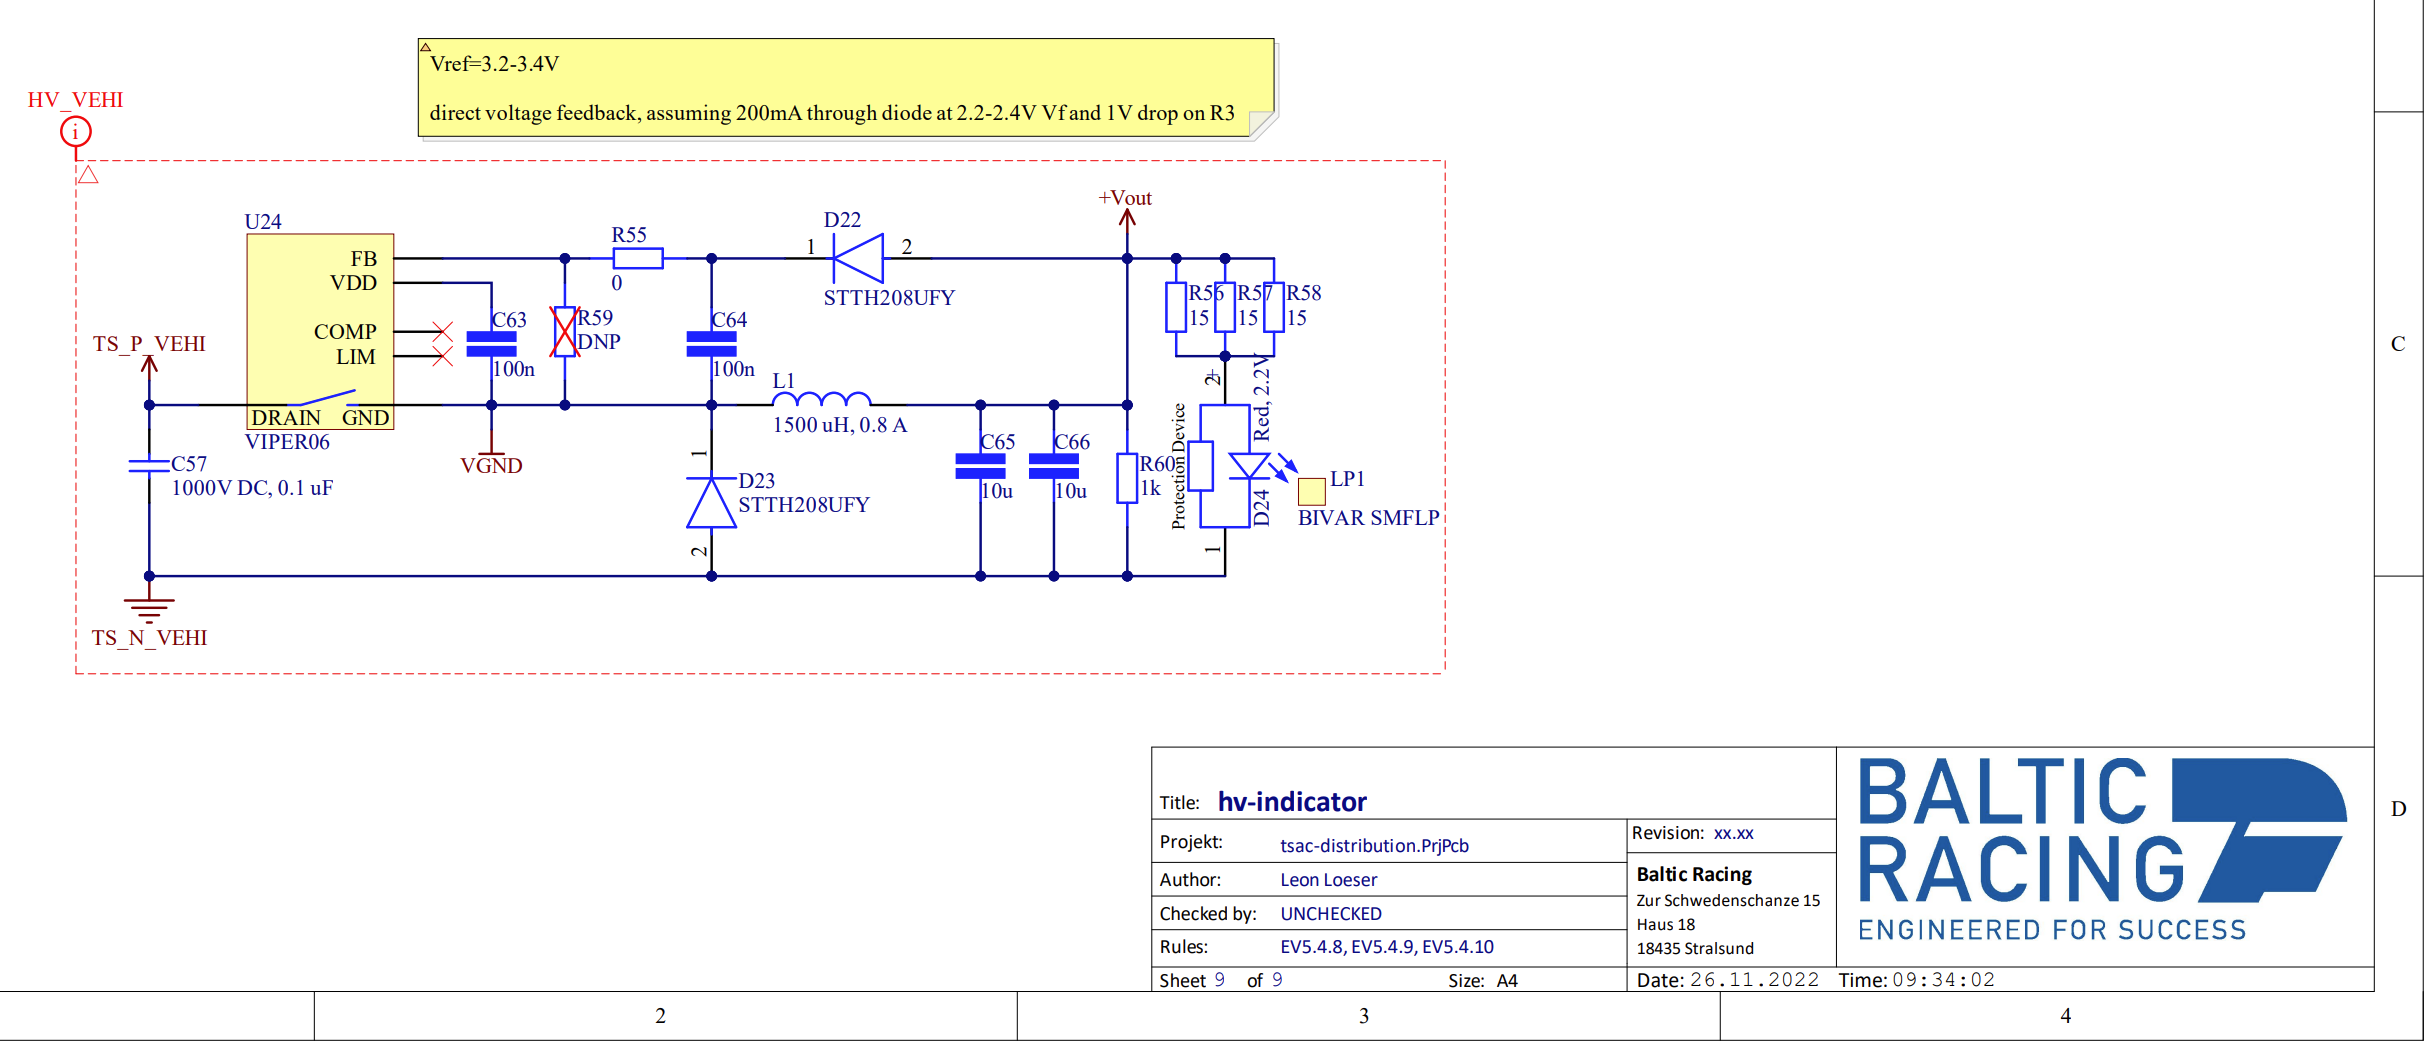
\includegraphics[width=0.7\linewidth]{bilder/HV_indicator_schematic}
	\caption{}
	\label{fig:hvindicatorschematic}
\end{figure}

Der HV Indikator ist ein rotes Licht auf dem Akkumulator, sofern an HV Terminals des Akkus eine gefährliche Spannung liegt muss dieses Licht erleuchten und dem Bediener somit anzeigen das es z.b. nicht sicher ist den Akku vom Zwischenkreis zu trennen da dieser noch unter Spannung steht. Die Anzeige erfolgt über eine Rote LED wessen licht mit einer Glasfaser von der Platine zum Deckel geleitet wird. Die Ansteuerung der LED erfolgt über einen kleinen DC Wandler, den Viper06. Dieser Wandler verfügt über einen Drain Source startup Voltage von 25-40V. Das bedeutet, bei einer Spannung in diesem Bereich beginnt der Chip zu arbeiten. Dieser Strom fließt dann zur LED so das diese zu leuchten beginnt. Die Feedback Schaltung ist direkt an den Spannungsausgang gekoppelt so das wir die interne Spannungsreferenz von 3,2 V - 3,4 V nutzen. Die Vorwiederstände vor der LED sind dementsprechend ausgelegt.

\FloatBarrier
\subsubsection{HV Messung}
Sinn der HV Messung ist es die Spannung welche am Akku als auch am Zwischenkreis anliegt erfassen und digitalisieren zu können. Dadurch kann zusammen mit dem Signal vom Stromsensor z.b. die DC Leistung bestimmt und geloggt werden. 

\begin{figure}
	\centering
	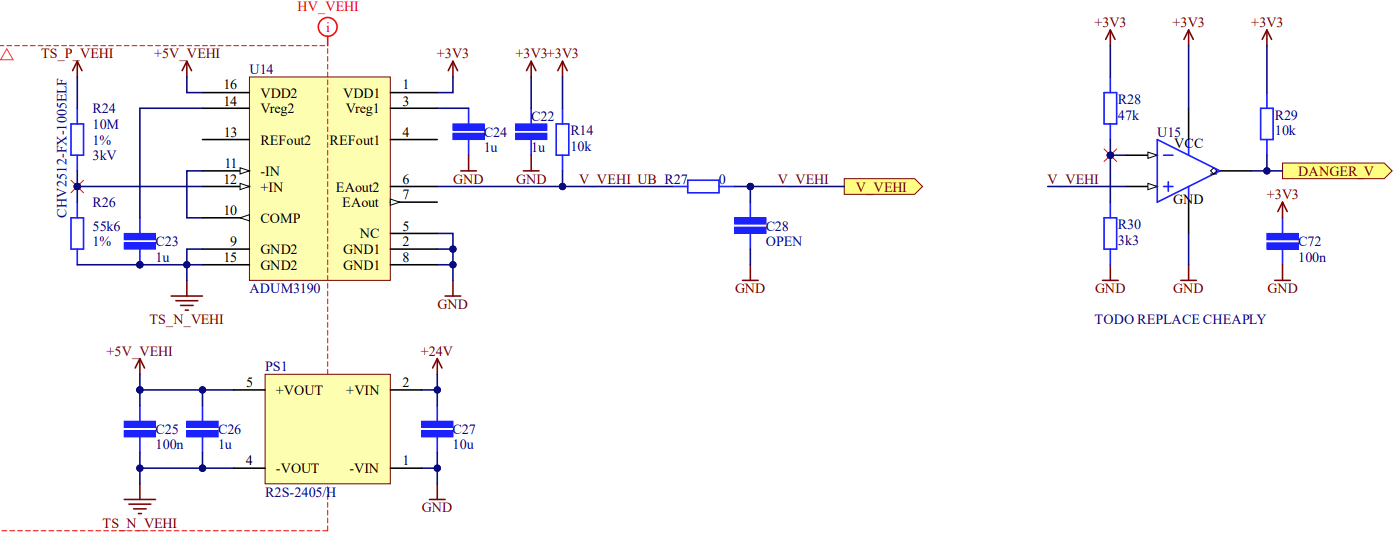
\includegraphics[width=0.7\linewidth]{bilder/HV_Measurement_PNG}
	\caption{}
	\label{fig:hvmeasurementpng}
\end{figure}

\begin{figure}
	\centering
	\includegraphics[width=0.4\linewidth]{"bilder/Blockdiagramm ADUM3190"}
	\caption{}
	\label{fig:blockdiagramm-adum3190}
\end{figure}

Kern dieser Schaltung ist der ADUM 3190. dabei handelt es sich um einen Isolierten Operationsverstärker. Der positive Eingang ist über einen Spannungsteiler mit dem HV-Kreis verbunden. Der negative Eingang ist mit dem Ausgang des OPV rückgekoppelt so das ein Spannungsfolger mit einer Verstärkung von 1 entsteht. Aus dem 10Mohm und dem 55,6kOhm widerstand ergibt sich eine Verhältnis von 179,86V im HV Kreis zu einem Volt am Eingang des OPV. Das ergibt eine maximale Eingangsspannung für die Schaltung von 593,54V da hierbei eine Ausgangsspannung von 3,3V erreicht wird. Bei dem R2S-2405/H handelt es sich um einen isolierten DC Wandler um den Chip HV seitig mit Strom zu versorgen. Die Komparatorschaltung um U15 gibt bei überschreiten der gefährlichen Spannung einen High Pegel aus. Die Spannung über den positiven Eingang der komparatorschaltung liegt bei 0,232V so das bei einer TS Spannung von größer 41,73V der High Pegel anliegen sollte. Laut Regelwerk sollte dieser Pegel spätestens bei 60V anliegen.

\FloatBarrier
\subsubsection{IMD Monitoring}



\FloatBarrier
\subsection{HV DCDC}
Visio blockmodell
Erklärung ACFC
Berechnung excel etwas aufhübschen und anhängen
Teilberechnungen erklären

\FloatBarrier
\section{HV Distribution}

\FloatBarrier
\subsection{TSMP}
Die Tractive System Measuring Points befinden sich seitlich am Fahrzeug wo auch der Hauptschalter zu finden ist. Sie stellen eine genormte Schnittstelle dar um mit einem Duspol, oder Multimeter an die Spannung des Tractive Systems gelangen zu können. Hierbei müssen laut Regelwerk geschirmte Bananenstecker eingesetzt werden. Weiter muss für die Buchsen am Fahrzeug eine Abdeckkappe oder Blindstecker vorgesehen werden. Zur Absicherung der TSMP müssen diese mit Widerständen in reihe an den HV Kreis angebunden werden. Das Regelwerk sieht hierbei in unserem Spannungsbereich 15k$\Omega$ vor. Der Kritische wert wonach die TSMP ausgelegt werden müssen ist das Leistungsrating, da diese auf kontinuierlichen Kurzschluss ausgelegt sein müssen.

Eine Formel zu Berechnung der Leistung am Widerstand ist folgende

\begin{equation}
	\label{eqn:Leistung am Wiederstand}
	\glsc{symb:P_elektrisch} = \glsc{symb:I}^{2} * \glsc{symb:R}
\end{equation}

Der Strom errechnet sich aus.

\begin{equation}
	\label{eqn:URI}
	\glsc{symb:U} = \glsc{symb:R}^{2} * \glsc{symb:I}
\end{equation}

Umgestellt nach I.

\begin{equation}
	\label{eqn:IUR}
	\glsc{symb:I} = \dfrac{\glsc{symb:U}} {\glsc{symb:R}}
\end{equation}

Da im Kurzschlussfall die Spannung über beide Widerstände anliegt, verdoppelt sich der Widerstand.

\begin{table}[h]
	\centering
	\begin{tabular}{|c|c|c|}
		\hline
		\multicolumn{3}{|c|}{Eingangsparameter} \\
		\hline
		\glsc{symb:R} & 15 & \ensuremath{k\Omega} \\
		\hline
		\glsc{symb:U} & 600 & \ensuremath{V} \\
		\hline
		\multicolumn{3}{|c|}{Ergebnisse} \\
		\hline
		\glsc{symb:I} & 20 & \ensuremath{mA} \\
		\hline
		\glsc{symb:P_elektrisch} & 12 & \ensuremath{W} \\
		\hline
	\end{tabular}
\end{table}

Daraus schlussfolgert sich das die 15k$\Omega$ Widerstände mit einem Leistungsrating von mindestens 12 W benötigt werden.

\FloatBarrier
\subsection{BSPD}

VAC Sensorboard
Logik
\begin{figure}
	\centering
	\includegraphics[width=0.7\linewidth]{"bilder/BSPD Blockdiagramm"}
	\caption{}
	\label{fig:bspd-blockdiagramm}
\end{figure}

Die Aufgabe des BSPD ist es das Fahrzeug in dem Fall einer Störung des Gaspedales in einen Sicheren zustand zu überführen. Hierfür wird der Strom zu den Umrichtern als auch der Bremsdruck gemessen und beim eintreten eines im Regelwerk definierten schwellwertes für das gleichzeitige auftreten beider Signale muss das abschalten des Antriebes erfolgen. Das Folgende Blockdiagramm soll einen Überblick über den signalfluss ermöglichen.

Bei den Eingangsignalen handelt es sich um analoge spannungen. Für Sigfnalaufbereitung oder auch Digitalisierung der Signale werden Schitds Trigger einbgesetzt, Die Logik besteht aus diversen Logikgattern und die Set/reset Schaltung besteht aus RC Gliedern mit nachgeschaltetetn schmidt triggern. Beim Shutdowncircuit handelt es sich um ein Solid State Relay welches von der BSPD Logik schlussendlich angestuert werden soll, ein öffnen des Shutdwon circuit führt damnit zu einem Herunterfahren des Antriebes.

Zur Auslegung von Schmidt Triggern
\begin{figure}
	\centering
	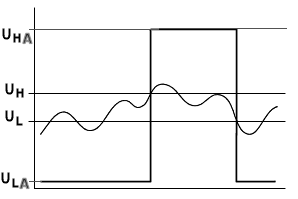
\includegraphics[width=0.5\linewidth]{bilder/Schmitt-trigger-diagramm.png}
	\caption{}
	\label{fig:schmitt-trigger-diagramm}
\end{figure}

Die Funktionsweise eines Schmitt Trigger kann anhand des Bildes erkannt werden. Er ermöglicht es ein analoges Signal in ein Digitales umzuwandeln, dabei ist es möglich festzulegen welche Spannungspegel am Ausgang des Schmitt Trigger anliegen (\glsc{symb:U_HA} und \glsc{symb:U_LA}) und bei welchen Spannungspegeln der Trigger High respektive Low schalten soll (\glsc{symb:U_H}und \glsc{symb:U_L}). Das vorliegen unterschiedilcher Pegel zum Schalten wird Hysterese genannt. Grund für das vorliegen ist das verhindern des rapiden Umschaltens zwischen High und Low direkt an dem Schwellwert aufgrund von Signalrauschen.

\begin{figure}
	\centering
	\includegraphics[width=0.7\linewidth]{"bilder/TPS Failure detection"}
	\caption{}
	\label{fig:tps-failure-detection}
\end{figure}

\begin{figure}
	\centering
	\includegraphics[width=0.5\linewidth]{"bilder/nichtinvertierender Trigger"}
	\caption{}
	\label{fig:nichtinvertierender-trigger}
\end{figure}

Folgend Beispielhaft die Auslegung eines Nicht Invertierenden Schmitt Triggers wie er im Bild unten zu sehen ist. Die andere Ausführung ist die eines Invertierenden.

Zur Berechnung sollten sich \glsc{symb:U_HA} und \glsc{symb:U_LA} sowie \glsc{symb:U_H} und \glsc{symb:U_L} aus dem Betriebsfall ergeben. R\textsubscript{1} sowie R\textsubscript{3} können frei gewählt werden. R\textsubscript{1} ist hierbei der Verbund aus R\textsubscript{3} und R\textsubscript{4}.

Die beiden folgenden Gleichung liegen zu Grunde

\begin{equation}
	\label{eqn:Obere Hysteresespannung Schmitt Trigger}
	\glsc{symb:U_H} = \glsc{symb:U_ref} + (\glsc{symb:U_HA} - \glsc{symb:U_ref}) * \dfrac{R\textsubscript{1}} {R\textsubscript{1}+R\textsubscript{2}}
	mit R\textsubscript{1}=\dfrac{R\textsubscript{3}*R\textsubscript{4}}{R\textsubscript{3}+R\textsubscript{4}}
\end{equation}

Und

\begin{equation}
	\label{eqn:Untere Hysteresespannung Schmitt Trigger}
	\glsc{symb:U_L}=\glsc{symb:U_ref}-(\glsc{symb:U_ref}-\glsc{symb:U_HA})*\dfrac{R\textsubscript{1}}{R\textsubscript{1}+R\textsubscript{2}}
\end{equation}

Mit den folgenden Gleichungen lassen sich R\textsubscript{2} und R\textsubscript{4} bestimmen

\begin{equation}
	\label{eqn:Berechnung R2 Schmitt Trigger}
	R\textsubscript{2} = R\textsubscript{1} * \dfrac{\glsc{symb:U_HA} - \glsc{symb:U_LA}} {\glsc{symb:U_H} - \glsc{symb:U_L}}
\end{equation}

\begin{equation}
	\label{eqn:Berechnung Uref Schmitt Trigger}
	\glsc{symb:U_ref} = (\glsc{symb:U_H} - \glsc{symb:U_LA}) * \dfrac{R\textsubscript{2}} {R\textsubscript{1} + R\textsubscript{2}} + \glsc{symb:U_LA}
\end{equation}

\begin{equation}
	\label{eqn:Berechnung R4 Schmitt Trigger}
	R\textsubscript{4} = R\textsubscript{3} * \dfrac{\glsc{symb:VCC}-\glsc{symb:U_ref}} {\glsc{symb:U_ref}}
\end{equation}

\begin{figure}
	\centering
	\includegraphics[width=0.7\linewidth]{"bilder/BSPD Integrator"}
	\caption{}
	\label{fig:bspd-integrator}
\end{figure}

Zur Auslegung der Zeitsteuerung

Die Zeitsteuerung besteht aus einem Kondensator C2 welcher über den Widerstand R20 geladen wird, einer Diode D3 um Rückkopplung zu vermeiden, einem Widerstand R23 um den Kondensator langsam zu entladen, einem Spannungsfolger OP2 um die Schaltung von dem nachgeschalteten Schmitt Trigger zu entkoppeln und einem Transistor T3 der den Kondensator in kurzer Zeit bei Bedarf entladen kann.

Für die Berechnung ist die Ladezeit des Kondensators über den Widerstand R20 bis zur Schaltspannung des Schmitt Triggers zu ermitteln. Dies lässt sich mit folgender Gleichung Lösen. 

\begin{equation}
	\label{eqn:Ladezeit Kondensator}
	\glsc{symb:U_a}=\glsc{symb:U_e}*(1-\glsc{symb:e}^{\dfrac{1}{\glsc{symb:R}*\glsc{symb:C}}*\glsc{symb:t}})
\end{equation}

Alternativ kann der Schmitt Trigger aber auch auf 0,63 fache der Eingangsspannung gesetzt werden was der einfachen Zeitkonstante des RC Gliedes entspricht. Damit bestimmt sich C wie folgt.

\begin{equation}
	\label{eqn:Zeitkonstante Kondensator}
	\glsc{symb:C}=\dfrac{\glsc{symb:tau}}{\glsc{symb:R}}
\end{equation}

Mit Beispielhaften Auslegeparametern ergeben sich folgende Werte.

\begin{table}[h]
	\centering
	\begin{tabular}{|c|c|c|}
		\hline
		\multicolumn{3}{|c|}{Eingangsparameter} \\
		\hline
		\glsc{symb:tau} & 0,5 & \ensuremath{s} \\
		\hline
		\glsc{symb:R} & 100 & \ensuremath{k\Omega} \\
		\hline
		\multicolumn{3}{|c|}{Ergebnisse} \\
		\hline
		\glsc{symb:C} & 5 & \ensuremath{uF} \\
		\hline
	\end{tabular}
\end{table}

Das BSPD-Sensorboard hat zum Zweck einen Stromsensor zu kreieren der ein Stromsignal von 0-100A in ein Spannungssignal von 0.5-4.5V über den Bereich von 0-10A zu erzeugen. Die 0.5V Offset haben zum ziel eine Kurzschlusserkennung auf Masse als auch auf Versorgung zu ermöglichen. Der relevante Messbereich von 0-10A entsteht aus den Regelwerksanforderungen die vorgeben das der Fehlerzustand bei einer abgerufenen Leistung größer 5kW eingestellt werden muss was bei 600V in einem Strom von 8,3A resultiert. Dieser Bereich muss möglichst robust ausgewertet werden können.

Zur genauen Funktion, U1 ist ein Hall Effekt Stromsensor mit einem Übersetzungsfaktor von 1000. Heißt 10A ergeben 10mA Stromfluss am Ausgang. Der Widerstand R2 ist so gewählt das bei einem Strom von 10mA, 5V über den Widerstand abfallen und wir so in den Messbereich kommen. Der Widerstand R1 ermöglicht nun das konstante einspeisen von ca. 0,5V und die Diode das Begrenzen der max. Spannung auf 4,5V.

\begin{figure}
	\centering
	\includegraphics[width=0.7\linewidth]{"bilder/Sensorboard Schaltung"}
	\caption{}
	\label{fig:sensorboard-schaltung}
\end{figure}

\FloatBarrier
\subsection{Discharge}
Die Discharge Schaltung soll bei Abschalten des Fahrzeug die Zwischenkreiskondensatoren entladen. Ziel ist es das System möglichst schnell in einen Spannungsfreien und damit sicheren Zustand zu überführen.
\begin{figure}
	\centering
	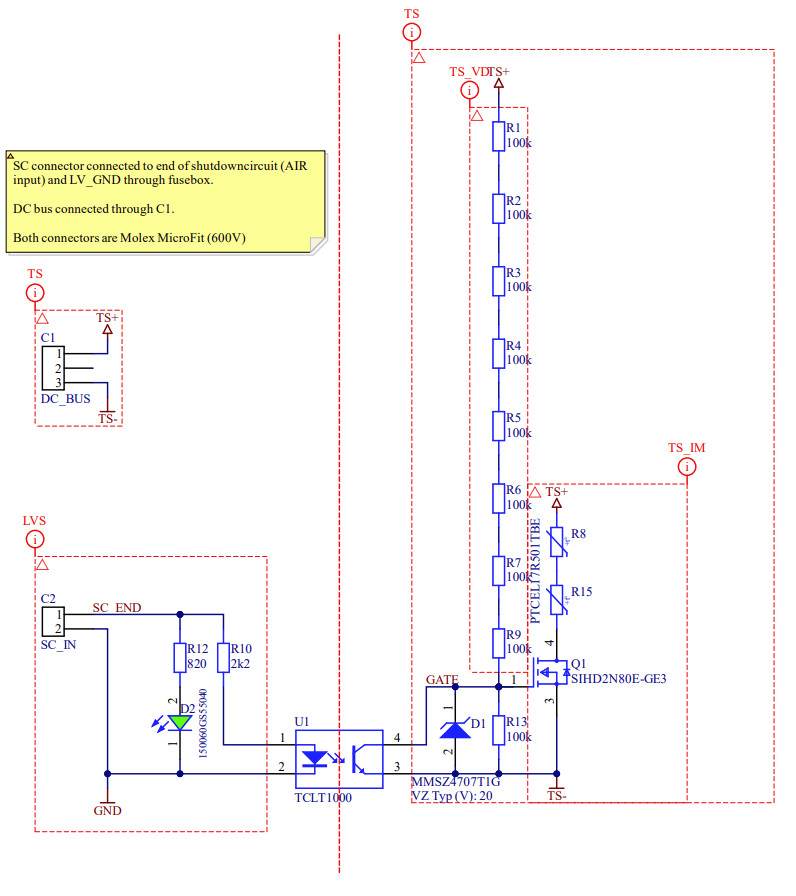
\includegraphics[width=0.7\linewidth]{bilder/Discharge}
	\caption{}
	\label{fig:discharge}
\end{figure}

Dies kann mit Hilfe von PTC Widerständen geschehen. Das Regelwerk sieht vor das der Zwischenkreis in maximal 5s auf 60VDC oder weniger zu bringen ist. Dies muss für 3 aufeinanderfolgende Entladevorgänge möglich sein. 

Die Ansteuerung erfolgt über den SDC welcher über den Steckverbinder C2 eingebunden ist. Von dort wird der Optokoppler U1 bestromt. Dieser Steuert Strom vom Gate des Mosfets Q1 weg Richtung TS- so das der Mosfet öffnet. Wenn der SDC geöffnet wird, steigt die Spannung am Gate auf 20V und der Mosfet steuert TS+ auf TS- über die PTC Wiederstände durch. Dadurch wird die Spannung im zwischenkreis in den PTC elementen abgebaut.

Die Formel für die Berechnung der PTC Elemenete ist dem Datenblatt für die PTCEL Serie der Firma Vishay zu entnehmen.

\begin{equation}
	\label{eqn:PTC Berechnung}
	\glsc{symb:N_PTC}=\dfrac{\glsc{symb:N_dump} * \glsc{symb:K} * \glsc{symb:C} * \glsc{symb:U}^{2}} {2 * \glsc{symb:R} * \glsc{symb:C_th} * (\glsc{symb:T_SW} - \glsc{symb:T_u})}
\end{equation}

\begin{table}[h]
	\centering
	\begin{tabular}{|c|c|c|c|}
		\hline
		\multicolumn{4}{|c|}{Eingangsparameter} \\
		\hline
		\glsc{symb:T_SW} & 130 & \ensuremath{°C} & Datenblatt Wiederstandsverlauf \\
		\hline
		\glsc{symb:K} & 1 & \ensuremath{-} & Datenblatt -> DC \\
		\hline
		\glsc{symb:C_th} & 2,3 & \ensuremath{J/K} & Datenblatt -> PTCEL17 \\
		\hline
		\glsc{symb:T_u} & 60 & \ensuremath{°C} & Worst Case \\
		\hline
		\glsc{symb:C} & 400 & \ensuremath{uF} & 2x DTI 500 Kapazität \\
		\hline
		\glsc{symb:U} & 600 & \ensuremath{V} & \\
		\hline
		\glsc{symb:N_dump} & 4 & \ensuremath{-} & min 3 Regelwerk\\
		\hline
		\multicolumn{4}{|c|}{Ergebnisse} \\
		\hline
		\glsc{symb:N_PTC} & 1,79 & \ensuremath{-} &  \\
		\hline
	\end{tabular}
\end{table}

Damit ergibt sich das 2 PTC`s des Typ 17R251 oder 17R501 verwendet werden müssen. 

Die Entladezeit kann wie beim BSPD über die bestimmt werden, in diesem Fall näherungsweise über die 3 fache Zeitkonstante. Damit ergibt sich eine Entladezeit von max. 1,2s.

\FloatBarrier
\section{TSAL}

\FloatBarrier
\subsection{Logik auf Discharge}
\label{sec: TSAL Logik Discharge}
\begin{figure}
	\centering
	\includegraphics[width=0.7\linewidth]{"bilder/Binäre Spannungserkennung"}
	\caption{}
	\label{fig:binare-spannungserkennung}
\end{figure}

Das Herz der Schaltung ist ein Verarmungstyp N-Fet. Wenn die Gate Source Spannung V\textsubscript{GS} = 0 V ist, dann lässt dieser Fet Strom durch. Ab einer Spannung von 47V wird die Zehner diode durchbrochen und ein Strom fließt, dieser Strom verursacht einen Spannungsabfall am Wiederstand R18 von ca. 2,2V bei einem mA so das V\textsubscript{GS} negativ wird und der Fet den Stromfluss zu begrenzen beginnt. Der Fet agiert zusammen mit dem Widerstand wie eine Konstantstromquelle. Diese Steuert den Optokoppler durch so das wir auf der LV Seite ein Signal erzeugt haben.

\FloatBarrier
\subsection{Logik auf AMS Master}

\FloatBarrier
\subsection{Schaltung auf TSAL}